%% report_progress.tex
%% Micromotion Simulation Project — Technical Report
%% Compile with: pdflatex report_v3 && bibtex report_v3 && pdflatex report_v3 && pdflatex report_v3
%%
\documentclass[english, 10pt, a4paper]{article}
\usepackage[T1]{fontenc}
\usepackage{lmodern}
\usepackage{geometry}
    \geometry
    {
        a4paper, 
        left    = 20mm,
        right   = 20mm,
        top     = 18mm,
        bottom  = 18mm,
    }
\usepackage{graphicx}
\usepackage{booktabs}
\usepackage{array}
\usepackage{multirow}
\usepackage{amsmath}
\usepackage{amssymb}
\usepackage{caption}
\usepackage{subcaption}
\usepackage{hyperref}
\usepackage{xcolor}
\usepackage{float}
\usepackage[protrusion=true, expansion=false]{microtype}
\usepackage{parskip}
\usepackage{enumitem}
\usepackage{siunitx}
\usepackage{fancyhdr}

% ── Path to figures ────────────────────────────────────────────────────────────
\graphicspath{{images/}}

% ── Colour definitions ─────────────────────────────────────────────────────────
\definecolor{flagred}{RGB}{192,0,0}
\definecolor{flagorange}{RGB}{230,126,0}
\definecolor{flaggreen}{RGB}{0,140,0}
\definecolor{flagblue}{RGB}{33,102,172}
\definecolor{flaggrey}{RGB}{100,100,100}

% Silence hyperref's complaints about \si{} in section headings/bookmarks
\pdfstringdefDisableCommands{%
 \def\si#1{#1}%
 \def\SI#1#2{#1\,#2}%
}

\hypersetup{
  colorlinks = true,
  linkcolor = flagblue,
  citecolor = flagblue,
  urlcolor  = flagblue,
}

% ── Column types ───────────────────────────────────────────────────────────────
\newcolumntype{L}[1]{>{\raggedright\arraybackslash}p{#1}}
\newcolumntype{C}[1]{>{\centering\arraybackslash}p{#1}}
\newcolumntype{R}[1]{>{\raggedleft\arraybackslash}p{#1}}

% ── Helpers ────────────────────────────────────────────────────────────────────
\newcommand{\flag}[2]{\textcolor{#1}{\textbf{[#2]}}}
\newcommand{\dZ}{\ensuremath{\delta Z}}
\newcommand{\dR}{\ensuremath{\delta R}}
\newcommand{\dX}{\ensuremath{\delta X}}
\newcommand{\Rb}{\ensuremath{R_b}}
\newcommand{\Cm}{\ensuremath{C_m}}
\newcommand{\dAlpha}{\ensuremath{\delta\alpha}}

\renewcommand{\thefootnote}{\alph{footnote}}
% ══════════════════════════════════════════════════════════════════════════════
\begin{document}

\begin{center}
 \centering
 {\LARGE\bfseries Decomposition of micromotion signals into physically interpretable perturbation modes via lattice based simulations}\\
 \textsc{Esteban Acerbo$^{1,3,4,}$\footnote[1]{Send any correspondence by email to: esteban.acerbo@ib.edu.ar - ORCID: 0000-0001-7021-5208}, Mariela I. Bellotti$^{1,2,5}$, Fabian J. Bonetto$^{1,2,3,4}$}\\
  \textsc{\small{$^1$ \textit{Laboratorio de Cavitación y Biotecnología, Centro Atómico Bariloche (CAB), Bariloche, Argentina.}\\$^2$ \textit{Comisión Nacional de Energía Atómica (CNEA), Centro Atómico Bariloche (CAB), Bariloche, Argentina}\\$^3$ \textit{Consejo Nacional de Investigaciones Ciencia y Técnicas (CONICET), Buenos Aires, Argentina.}\\$^4$ \textit{Universidad Nacional de Cuyo - Instituto Balseiro, Bariloche, Argentina.}}\\$^5$ \textit{Centro Patagónico Interdiciplinario de Investigaciones en Salud (CePIIeS), Bariloche, Argentina.}} \\[0.5cm]
 {\normalsize \today}\\[1cm]
\end{center}
 \begin{abstract}
  \noindent
Confluent cell monolayers over electrodes exhibit continuous impedance fluctuations that encode morphological and mechanical information at sub-second timescales, driven by lateral displacements, tight-junction remodeling, and biophysical parameter space heterogeneity. Decomposing these fluctuations into their constituent physical mechanisms remains an open problem, as each time step provides only two scalar observables while the underlying state space is high-dimensional. This work addresses the signal reconstruction through physically parameterized lattice-based simulation libraries built on a finite-difference model sharing the Giaever and Keese analytical model parametrization. Four perturbation libraries were computed, representing electrode-monolayer relative movement, subcellular tight-junction geometry modification, collective brick-wall rearrangement, and biophysical parameter microperturbations. Together, these libraries cover the experimental phase space for four physiological states: cell seeding, confluence, electrical wound healing, and post-healing confluence. Two reconstruction algorithms were evaluated: a greedy nearest-prototype method that assigns one mode per library per time step by sequentially minimizing the running residual, and a sparse Viterbi algorithm that enforces smooth state trajectories at the cost of fit quality. Both produce physically interpretable, model-consistent state sequences for each experimental electrode.
\end{abstract}

% ══════════════════════════════════════════════════════════════════════════════
\section{Introduction}
\label{sec:intro}

Understanding individual and collective cell movement provides direct insight into the biochemical and mechanical signals underlying tissue formation, from embryogenesis to organ morphogenesis, and the dysregulation that drives pathological processes including cancer invasion and metastasis \cite{trepat2009physical, matoz2017cell}. Confluent epithelial monolayers exhibit collective dynamics analogous to liquids approaching a glass transition, displaying spatial heterogeneities \cite{matoz2017cell,henkes2020dense} and back and forth oscillations \cite{petrolli2019confinement}. In the field of monolayer monitoring Electric Cell-substrate Impedance Spectroscopy (ECIS) technique provides a continuous, non-invasive readout of the collective state of a cell monolayer adhered to a planar gold electrode by monitoring its spectral impedance. In addition, by monitoring the cell monolayer at sub-second resolution with a fixed excitation frequency, ~\cite{giaever1991micromotion,giaever1993biosensor, keese1994biosensor,giana2018desarrollo} the impedance evolution reveals the collective correlated cell movement or micromotion, as signal fluctuations providing of morphological and toxicity information \cite{giaever1989fractal,lovelady2009detecting, tarantola2011toxicity,izzard1980formation, acerbo2024determining}. 

The objective of this project is to decompose the impedance experimental micromotion time series into physically interpretable contributions from discrete perturbation modes, producing a state sequence that describes the dominant physical mechanism at each time step. The dataset analyzed here was originally reported in \cite{acerbo2024determining} as part of a quantitative fractal characterization of MDCKII monolayer cultures; the present work re-examines those recordings through the lens of the numerical simulation framework extending the Giaever-Keese analytical model. From the original dataset four micromotion time series were selected, all measured at \SI{1}{kHz} excitation frequency, which proved to be the most sensitive to culture-condition changes. The \SI{1}{kHz} value refers to the excitation frequency of the lock-in amplifier, not to the temporal sampling rate; the sampling interval ranges from \SI{0.19}{s} to \SI{0.27}{s} across recordings. Prior to each micromotion recording, a full spectral impedance sweep is acquired, from which the GK biophysical parameters ($\alpha$, $R_b$, $C_m$) of the confluent monolayer are obtained by fitting Eq.~\ref{Eq:Zcov}; these values define the baseline for the perturbation libraries and the spectral comparison in Fig.~\ref{fig:baseline}. No spectral information is available during the micromotion recording itself.

All signals were adaptively detrended by subtracting a centered moving-average filter with window $W$ from the raw $R(t)$ and $X(t)$ signals. This acts as a local high-pass filter, preserving fluctuations at timescales shorter than $W$ while removing slow drift. The window is group-adaptive: $W = 900$\,s for confluent and post-healing recordings, and $W = 300$\,s for seeding and wound-healing recordings, where the impedance rises monotonically over the measurement period and a shorter window is required to track the non-linear baseline. A moving average was preferred over global linear detrending because the wound-healing and seeding impedance trajectories are markedly non-linear over the multi-hour recording span; a single regression line cannot track the sigmoid wound recovery and leaves systematic, correlated residuals. The present work focuses on collective micromotion phenomena at sub-minute timescales, where the additive small-perturbation hypothesis underlying the libraries holds; longer-timescale processes such as macroscopic culture reorganization fall outside the current scope. The resulting fluctuation signals are stored as $\delta R(t)$ and $\delta X(t)$ for statistical analysis.
\begin{figure}[H]
  \centering
  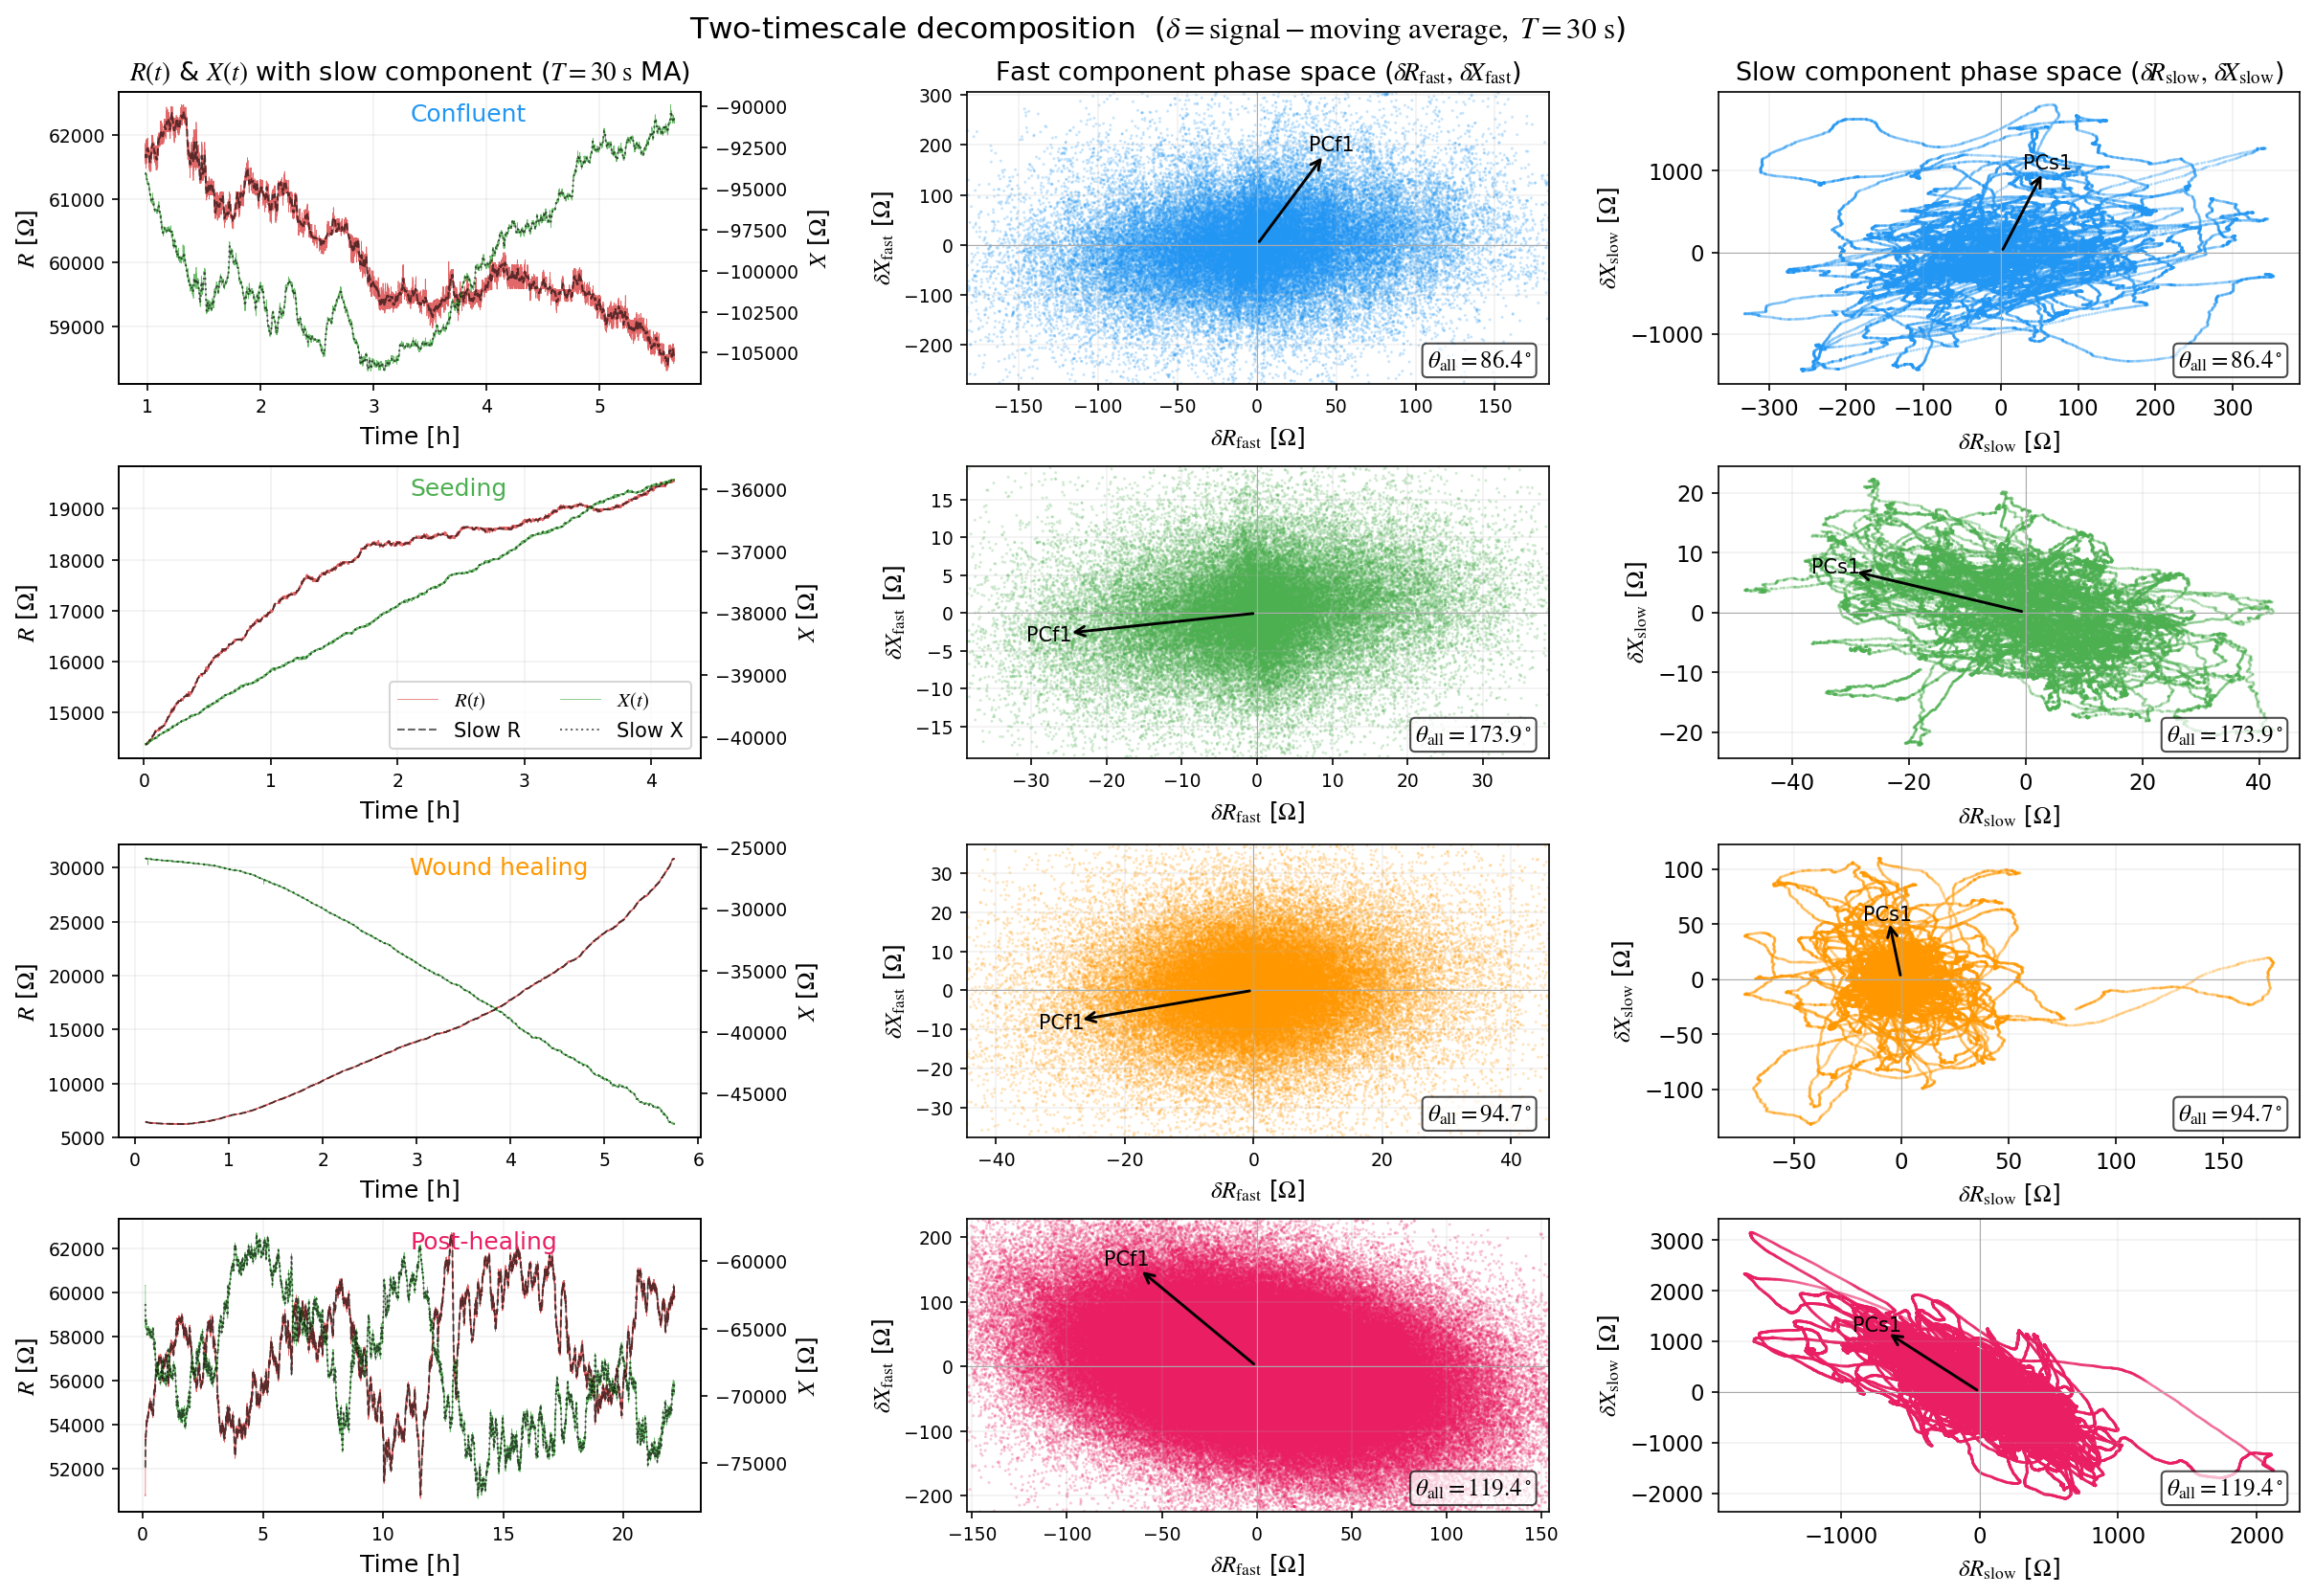
\includegraphics[width=1\linewidth]{figure1.png}
  \caption{Two-timescale decomposition of the four culture conditions (rows: seeding, confluent, wound healing, post-healing). The raw $R(t)$ and $X(t)$ signals are adaptively detrended to obtain $\delta R(t)$ and $\delta X(t)$; a second moving average ($T_\text{cut} = \SI{30}{s}$) separates fast ($<30$\,s) and slow ($>30$\,s) components. \textbf{Left column:} raw $R(t)$ (red) and $X(t)$ (green) time series with the slow component overlaid as dashed lines. \textbf{Central column:} fast-component phase space $(\delta R_\text{fast}, \delta X_\text{fast})$ with PC1 arrow and principal-axis angle $\theta_\text{PC}$. \textbf{Right column:} slow-component phase space $(\delta R_\text{slow}, \delta X_\text{slow})$ with PC1 arrow and $\theta_\text{PC}$.}
  \label{fig:timescales}
\end{figure} 

Principal component analysis (PCA) diagonalises the covariance matrix of $(\delta R,\delta X)$, yielding a principal axis angle $\theta_\text{all}$ (measured from the positive $\delta R$ axis, CCW positive) and standard deviations $s_1 \geq s_2$ along and perpendicular to that axis. A moving-average filter of width $T_\text{cut} = \SI{30}{s}$ further decomposes each signal into a fast component ($< 30$\,s, capturing individual cell micromotion events) and a slow component ($> 30$\,s, capturing collective reorganization), with PCA applied separately to each, as shown in Fig.~\ref{fig:timescales}. For seeding and wound-healing, the fast and slow principal-axis angles are nearly identical, indicating that a single dominant mechanism operates across all timescales. The post-healing recording is the sole exception, exhibiting a clear angular separation between timescales.

To characterize if the fractal scaling is homogeneous across timescales, two time-domain algorithms are therefore applied to decompose and cross-validate the scaling behavior across timescales: the Higuchi~\cite{higuchi1988approach, nobukawa2019atypical} algorithm and Rescaled Range (R/S) analysis~\cite{feder1988fractalChapter8, lloyd1966long, RSrepository}, both described in the previous work \cite{acerbo2024determining}. These estimates are obtained from the fully detrended $\delta R(t)$ and $\delta X$ signals; they are not directly comparable to the values reported which were computed on raw, non-detrended impedance trajectories. Each signal is divided into analysis windows of 12\,500 points and for each window the algorithm's log-log scaling curve is computed, obtaining the statistical fractal dimention \cite{guyonnet2019statistics, brewer2006limitations}. For the Higuchi method, the log-log curves of all windows were averaged and a single breakpoint was located by minimising the total piecewise residual sum of squares; the breakpoint was then forced on each individual window to extract fast-timescale ($D_f^\text{fast}$) and slow-timescale ($D_f^\text{slow}$) slopes separately. R/S was treated with a single slope only, as its lag-range structure does not admit a reliable piecewise decomposition.

The results are summarised in Table~\ref{tab:fractal_dim}. For $\delta R$, fractal dimension estimates are consistently high across almost all states (Higuchi single-slope range 1.67–1.87). Post-healing yields the lowest values ($1.67 \pm 0.04$ Higuchi, $1.43 \pm 0.04$ R/S), indicating a measurable reduction in signal complexity following to culture wound closure and radial cell reordening \cite{gamal2015real}, while Seeding and Wound healing are comparable ($\approx 1.87$ and $1.86$ by Higuchi), suggesting similar short-term fluctuation structure in both poorly-confluent and actively remodeling cultures. The Higuchi breakpoint decomposition of $\delta R$ consistently reveals a fast segment exceeding the slow segment, indicating that short-timescale dynamics are geometrically more complex. For $\delta X$, a sharper contrast between states emerges. Seeding records a near-Brownian dimension of $1.920 \pm 0.006$, while Confluent and Post-healing drop to $1.43 \pm 0.03$ and $1.40 \pm 0.02$ respectively, consistent with reactance fluctuations becoming smoother as the monolayer matures and membrane dynamics become collectively constrained. Wound healing is a notable exception, Higuchi and R/S, both with standard deviations larger than those of any other state or signal combination. This elevated dispersion across windows indicates that the $\delta X$ fractal scaling is not stationary during the wound-healing phase, likely reflecting the spatial heterogeneity, migrating cells, and intact monolayer coexist and contribute incoherently to the measured reactance fluctuations. The Higuchi breakpoint columns for Wound healing $\delta X$ should therefore be interpreted with caution, as the forced-split procedure finds an unstable inflection on an already variable averaged curve. 
 
\begin{table}[H]
 \centering
 \caption{Fractal dimension of $\delta R$ and $\delta X$ estimated by two algorithms. Values are mean $\pm$ standard deviation across analysis windows. Single: full-range slope; Fast: short-timescale segment; Slow: long-timescale segment at forced breakpoint. R/S fast and slow values are omitted as the forced breakpoint is not suited to the R/S scaling structure.}
 \label{tab:fractal_dim}
 \scriptsize
 \begin{tabular}{lcccccccccccc}
  \toprule
  & \multicolumn{4}{c}{$\delta R$} & \multicolumn{4}{c}{$\delta X$} \\
  \cmidrule(lr){2-5} \cmidrule(lr){6-9}
  Culture state & \multicolumn{3}{c}{Higuchi} & R/S & \multicolumn{3}{c}{Higuchi} & R/S \\
  \cmidrule(lr){2-4} \cmidrule(lr){6-8}
   & Single & Fast & Slow & Single & Single & Fast & Slow & Single \\
  \midrule
  Seeding & $1.87 (3)$ & $1.91 (2)$ & $1.77 (5)$ & $1.80 (2)$ & $1.920 (6)$ & $1.950 (2)$ & $1.83 (2)$ & $1.78 (2)$ \\
  Confluent & $1.81 (3)$ & $1.85 (2)$ & $1.75 (6)$ & $1.74 (3)$ & $1.43 (3)$ & $1.68 (5)$ & $1.39 (3)$ & $1.43 (4)$ \\
  Wound healing & $1.86 (3)$ & $1.91 (2)$ & $1.80 (4)$ & $1.78 (3)$ & $1.8 (1)$ & $1.92 (5)$ & $1.7 (1)$ & $1.66 (8)$ \\
  Post-healing & $1.67 (4)$ & $1.78 (3)$ & $1.52 (5)$ & $1.43 (4)$ & $1.40 (2)$ & $1.69 (2)$ & $1.33 (2)$ & $1.38 (3)$ \\
  \bottomrule
  \end{tabular}
  \end{table}


% ══════════════════════════════════════════════════════════════════════════════
\section{Bioimpedance Models}
\label{sec:model}

Giaever and Keese developed a model to quantify the biophysical properties of a confluent monolayer from its impedance spectrum~\cite{giaever1991micromotion,giaever1984monitoring}. The model derives the specific impedance of a cell-covered electrode under the assumption that every cell on the electrode is surrounded by identical neighbors, so that the radially symmetric current balance for a single representative cell can be integrated over the electrode area. The resulting specific impedance of the confluent monolayer is given by Eq.~\ref{Eq:Zcov}.
\begin{equation} \label{Eq:Zcov}
 \frac{1}{Z_\text{cov}} = \frac{1}{Z_n(Z_n+Z_m)}
 \left[Z_n + \frac{Z_m}{\dfrac{\gamma r_c}{2}
 \dfrac{I_0(\gamma r_c)}{I_1(\gamma r_c)}
 + R_b\!\left(\dfrac{1}{Z_n}+\dfrac{1}{Z_m}\right)}\right].
\end{equation}
With $I_i$ are the i-th modified Bessel function of first kind, $Z_n$ the specific impedance of the bare electrode, $Z_m(C_m)$ the membrane-specific impedance, $R_b$ the specific tight-junction resistance and $r_c$ the cell radius. For experimental data fitting it is convenient to define $\alpha = r_c\sqrt{\rho/h}$, where $\rho$ is the medium resistivity and $h$ the cleft height. Consequently, the specific impedance of the cell-covered electrode is characterized by three parameters, $\alpha$, $R_b$, and $C_m$.

The specific impedance of the bare electrode that enters Eq.~\ref{Eq:Zcov} as $Z_n$ is modelled as a constant-phase element (CPE):
\begin{equation}
 Z_n = Z_\text{CPE} = \frac{1}{A\,(j\omega)^n}. \label{Eq:CPE}
\end{equation}
A constriction resistance $R_\text{constr}$, introduced by the finite electrode geometry, is determined independently from the bare electrode spectrum and added in series only when comparing model predictions to experimental two-electrode data (Fig.~\ref{fig:baseline}); it does not enter the GK model, the simulation engine, or the perturbation libraries.

The simulation engine used in this work is a numerical finite-difference model based on the Giaever-Keese current balance approach, accounting for the electrode size and enabling the simulation of asymmetric cultures in fixed states snapshots. The simulated culture confluent construction over the electrode can be seen in Fig~\ref{fig:baseline} with the spectral impedance estimation, compared to experimental confluent data and the Giaever and Keese estimation using the same input parameters. The circular electrode of diameter \SI{350}{\mu m} (96W1E+ PET Applied Biophysics CultureWare) is centered on the domain. The culture is composed of square cells divided into sub-cellular square-pixel membrane tiles with a shared one-pixel-wide tight-junction ring at cell boundaries. For each square pixel the lateral and apical voltage differences are calculated enabling the passage of current from one cell cleft space in to the neighbors, this passage presents an impedance proportional to $\alpha$. Each pixel is assigned an apical impedance resistive ($\propto R_b$) or capacitive ($\propto C_m$) depending on being tight junction or interior membrane. The finite-difference voltage balance is solved for each pixel at each frequency, from which the electrode impedance is integrated. The parameters used throughout are $\alpha = 19.4 \pm 1.1$, $R_b = (14.4 \pm 2.0)\,\si{\ohm\centi\meter^2}$, and $C_m = (4.95 \pm 0.12)\,\si{\micro\farad\per\centi\meter^2}$, obtained from a spectral fit to a confluent MDCKII monolayer using Eq.~\ref{Eq:Zcov}. Although the finite-difference model uses square cells rather than the cylindrical cells of the GK model, no geometric conversion is required: the current balance is solved numerically on the pixel grid without assuming circular symmetry, and the biophysical parameters from the analytical GK fit are used directly. The small residual differences visible in Fig.~\ref{fig:baseline} arise from features resolved by the numerical model, namely current migration through the cleft to the insulating substrate and the finite pixel width of tight junctions, while the parametric sensitivity structure of the analytical model is conserved.

\begin{figure}[t]
  \centering
  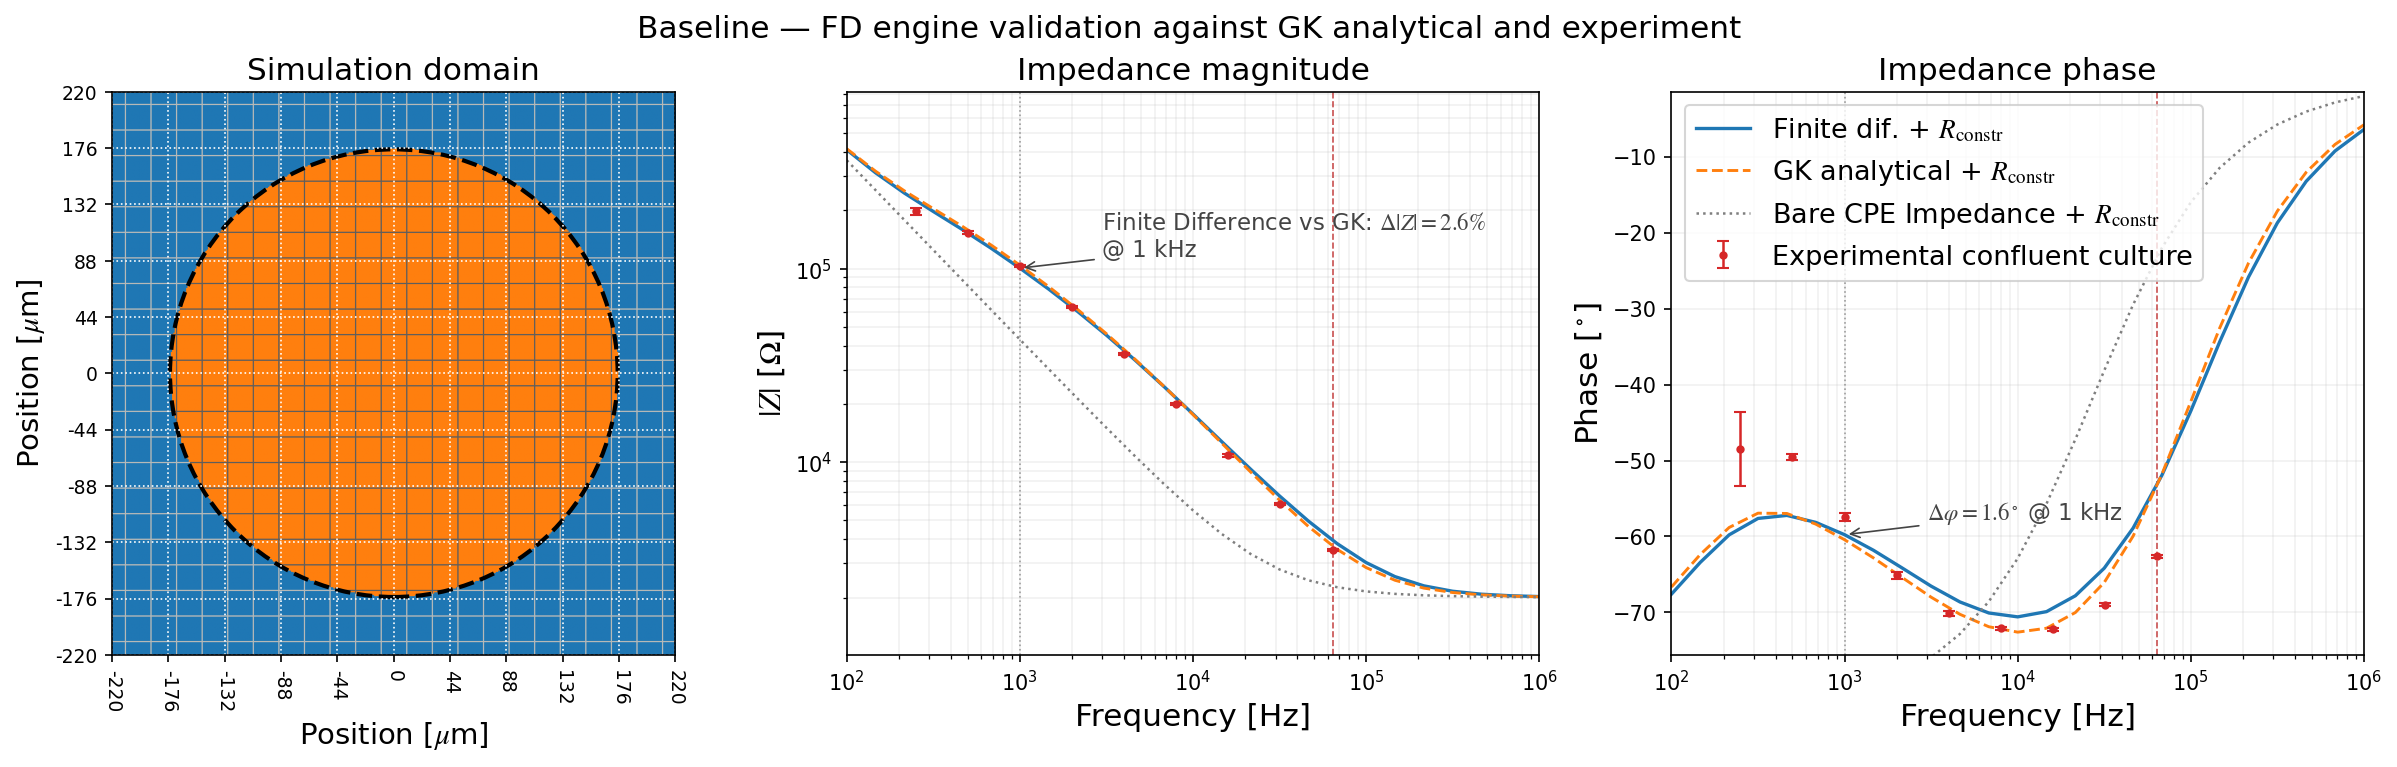
\includegraphics[width=\linewidth]{figure2.png}
  \caption{Finite-difference simulation construction and spectral impedance estimation. \textbf{Left:} Simulation domain showing the confluent square-cell culture map over the circular electrode. \textbf{Center:} Impedance modulus $|Z|(f)$ and \textbf{Right:} phase angle $\angle Z(f)$; each panel overlays the finite-difference result, the Giaever-Keese analytical model (Eq.~\ref{Eq:Zcov}) evaluated with the same parameters, experimental confluent MDCKII data, and the bare electrode modeled as a CPE. The 96W1E+ PET Applied Biophysics CultureWare consist in two identical electrodes. The total cultureware impedance result in the sum of two GK monolayers plus a constriction resistance or two finite difference simulations plus the constriction resistance. Each simulation or model estimation is based in half the bare electrode total impedance.}
  \label{fig:baseline}
 \end{figure}

The simulation framework is built on a fixed spatial lattice in which cell identities are assigned to pixel positions rather than tracked as individual mobile agents. This design rests on two complementary principles. The impedance measured at the electrode is determined by the aggregate spatial distribution of membrane, junction, and bare substrate pixels; permutation of two cells across the lattice leaves the impedance spectrum invariant, so tracking individual cell trajectories would expand the sampled hyperspace without adding observational content. Moreover, each impedance evaluation requires a full sparse finite-difference solve of the electrode boundary-value problem, making continuous-dynamics simulation computationally prohibitive at the required frequency resolution; the library approach replaces trajectory integration with a finite set of static equilibrium geometries whose impedance responses are pre-computed once and reused during reconstruction.

\section{Perturbation Libraries}
\label{sec:libraries}

Four deterministic libraries were computed by systematically modifying the confluent construction described above, each spanning a specific physical mechanism; no stochastic component enters the library construction or the reconstruction. Each mode stores the full impedance spectrum over 25 log-spaced frequencies from 100\,Hz to 1\,MHz, and the $(\delta R, \delta X)$ values are computed as the impedance deviation from the confluent baseline (Fig.~\ref{fig:baseline}). The libraries stand for independent additive small perturbations, taking the confluent baseline to the micromotion specific state, covering the experimental phasespace.

The first implemented simulations, Library~A represents a rigid translation of the monolayer grid over the electrode disc to represent culture oscillations. As the monolayer shifts, the mapping of tight-junction and membrane pixels onto the electrode integration domain changes while the electrode geometry and CPE parameters remain fixed. Simulations span a lower-triangular matrix sweep $\Delta x \in [0,40]$\,px, $\Delta y \in [0,\Delta x]$, exploiting the reflection symmetry of a square cell on a circular electrode to avoid redundant modes. The perturbation direction at \SI{1}{kHz} is consistently $(+\dR, -\dX)$, as seen in Fig.~\ref{fig:libA}.

\begin{figure}[t]
 \centering
 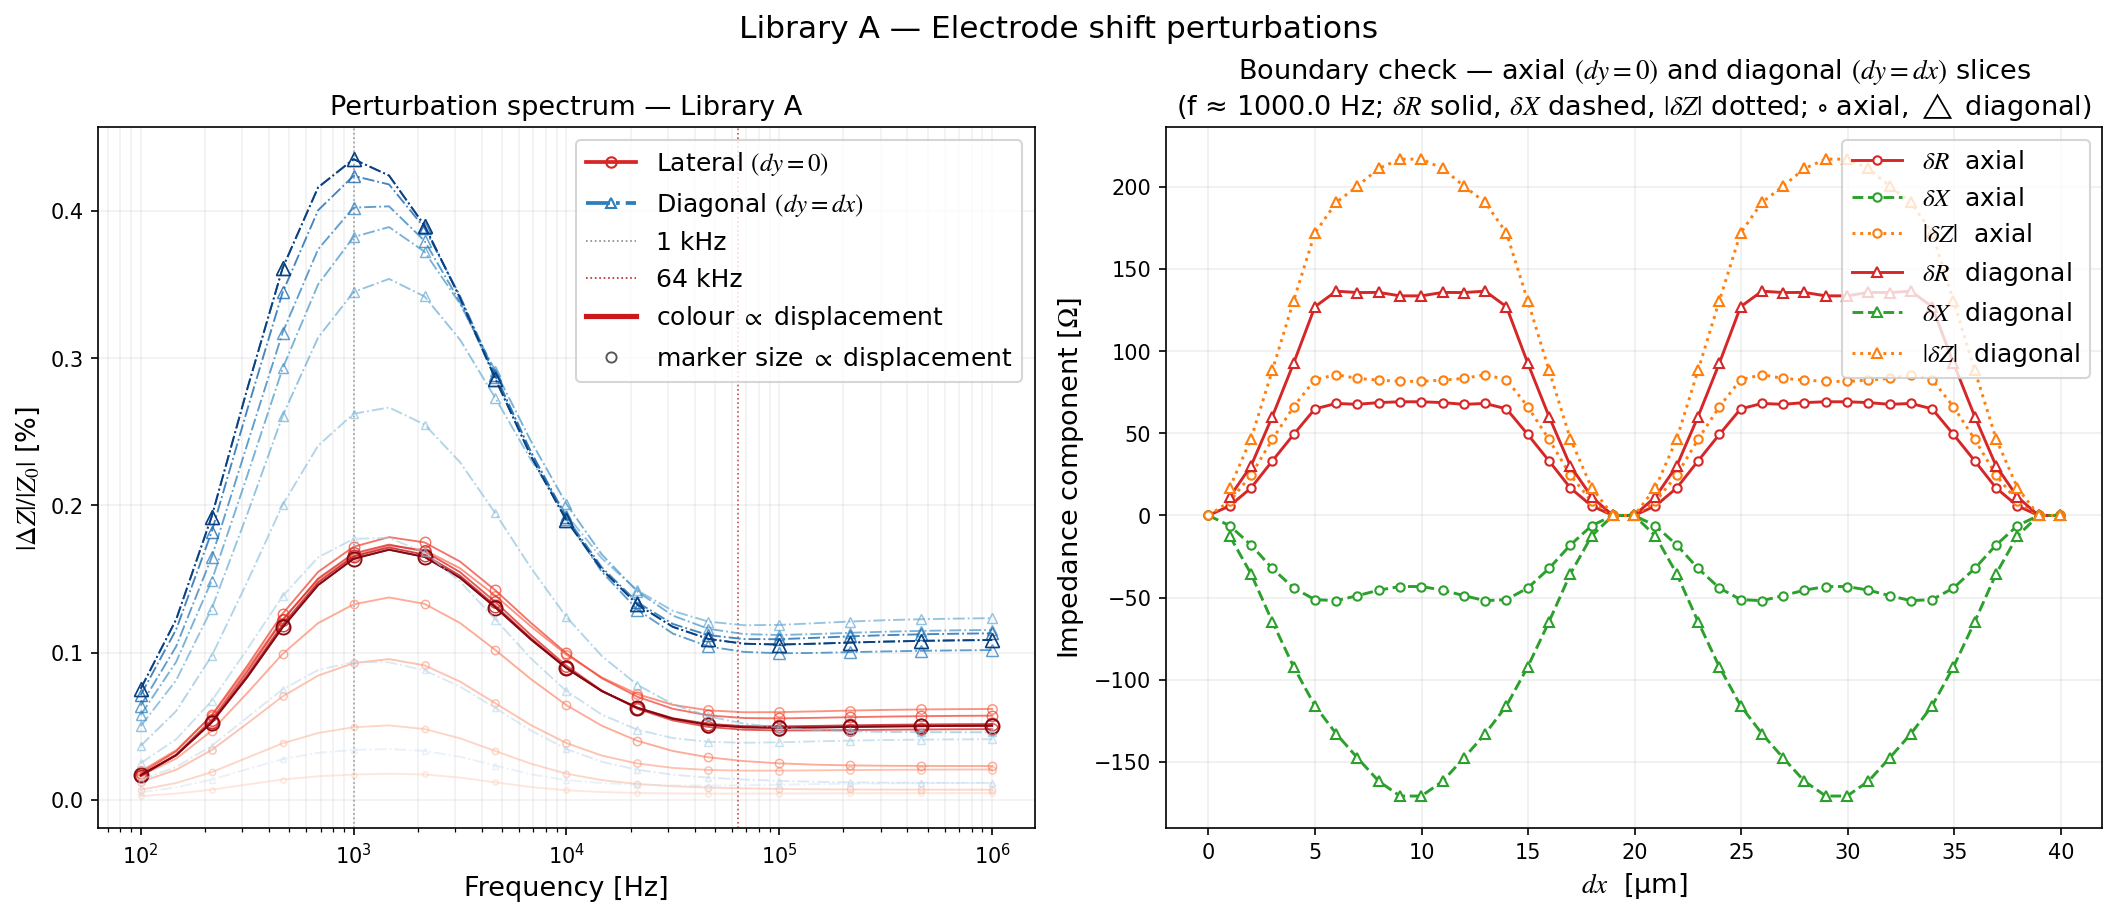
\includegraphics[width=\linewidth]{figure3.png}
 \caption{Library~A electrode-shift perturbations. \textbf{Left:} Normalized perturbation magnitude $|\Delta Z|/|Z_0|$ (\%) as a function of frequency for the lateral-shift and diagonal-shift series; line color and marker size increase with displacement magnitude. \textbf{Right:} Real part $\dR$, imaginary part $\dX$, and magnitude $|\delta Z|$ at \SI{1}{kHz} as a function of lateral or diagonal displacement $dx$ (\si{\micro\meter}), shown as separate overlaid curves for the lateral and diagonal series.}
 \label{fig:libA}
\end{figure}

Library~B models the systematic widening of cell junctions driven by intercellular mechanical tension, in which cells deform collectively along a common direction. Each cell simultaneously converts an L-shaped group of membrane pixels in one corner into tight-junction ($R_b$) type; the modification occupies $l_w$ pixels along both the horizontal and vertical arms, ranging from one pixel to half the cell side ($l_w \leq l_{w,\max}/2 = 9$ pixels). The circular symmetry of the electrode makes the choice of corner unimportant. A coupling parameter $K_{RB}$ rescales the tight-junction resistance in proportion to the arm length as defined in Eq.~\ref{Eq:Krb}, linking the geometric modification to the tight-junction impedance: positive $K_{RB}$ represents tension-induced junction tightening, while negative values model junction loosening. Because the fraction of cells deforming along a common direction in the real monolayer is unknown, multiple $K_{RB}$ values are tested, generating a 2D fan of perturbation directions in the $(\dR, \dX)$ plane.
\begin{equation} \label{Eq:Krb}
  R_b(l_w) = R_{b,0}\,\bigl(1 + K_{RB}\, l_w / l_{w,\max}\bigr),
\end{equation}
where $R_{b,0}$ is the baseline junction resistance, $l_w$ is the L-corner arm length in pixels, and $l_{w,\max}$ is the maximum possible interior arm length, equal to the cell side length in pixels.

Library~C models a collective geometric rearrangement associated with glassy monolayer dynamics, in which alternating cell columns are shifted vertically by a pixel offset. This transforms the square packing geometry toward a brick-wall pattern without altering the pixel-level membrane or junction conductances, and therefore without altering individual cell properties; the impedance change arises solely from the modified current-path topology, which is captured by re-solving the finite-difference balance on the rearranged geometry. The perturbation direction at \SI{1}{kHz} is consistently $(+\dR, +\dX)$, making it the only library that provides a positive contribution in both impedance components.

Library~D represents collective perturbations that produce impedance fluctuations without any geometric rearrangement: every cell on the electrode receives the same fractional parameter change, so the perturbed $\alpha$, $R_b$, and $C_m$ values represent effective culture-wide quantities. Changes in the cell--substrate cleft geometry or paracellular barrier properties translate directly into variations of these parameters. The library is constructed from the Cartesian product of fractional perturbation levels in $[-1\%,\,+1\%]$ for each of the three parameters, yielding a cube in the three-dimensional $(\delta\alpha,\,\delta R_b,\,\delta C_m)$ parameter space. When projected onto the two-dimensional $(\dR, \dX)$ observation plane at \SI{1}{kHz} (Fig.~\ref{fig:libD}, right), the modes cover regions in all four quadrants. The right panel displays the 12 edges of this projected cube, obtained by sweeping one parameter while the other two are held at their extreme values; the interior of the enclosed region contains the remaining modes. In this projection, $\delta\alpha$ perturbations map predominantly along the vertical ($\dX$) direction, $\delta C_m$ perturbations act nearly horizontally ($\dR$), and $\delta R_b$ perturbations translate diagonally across the phase space.

\begin{figure}[H]
 \centering
 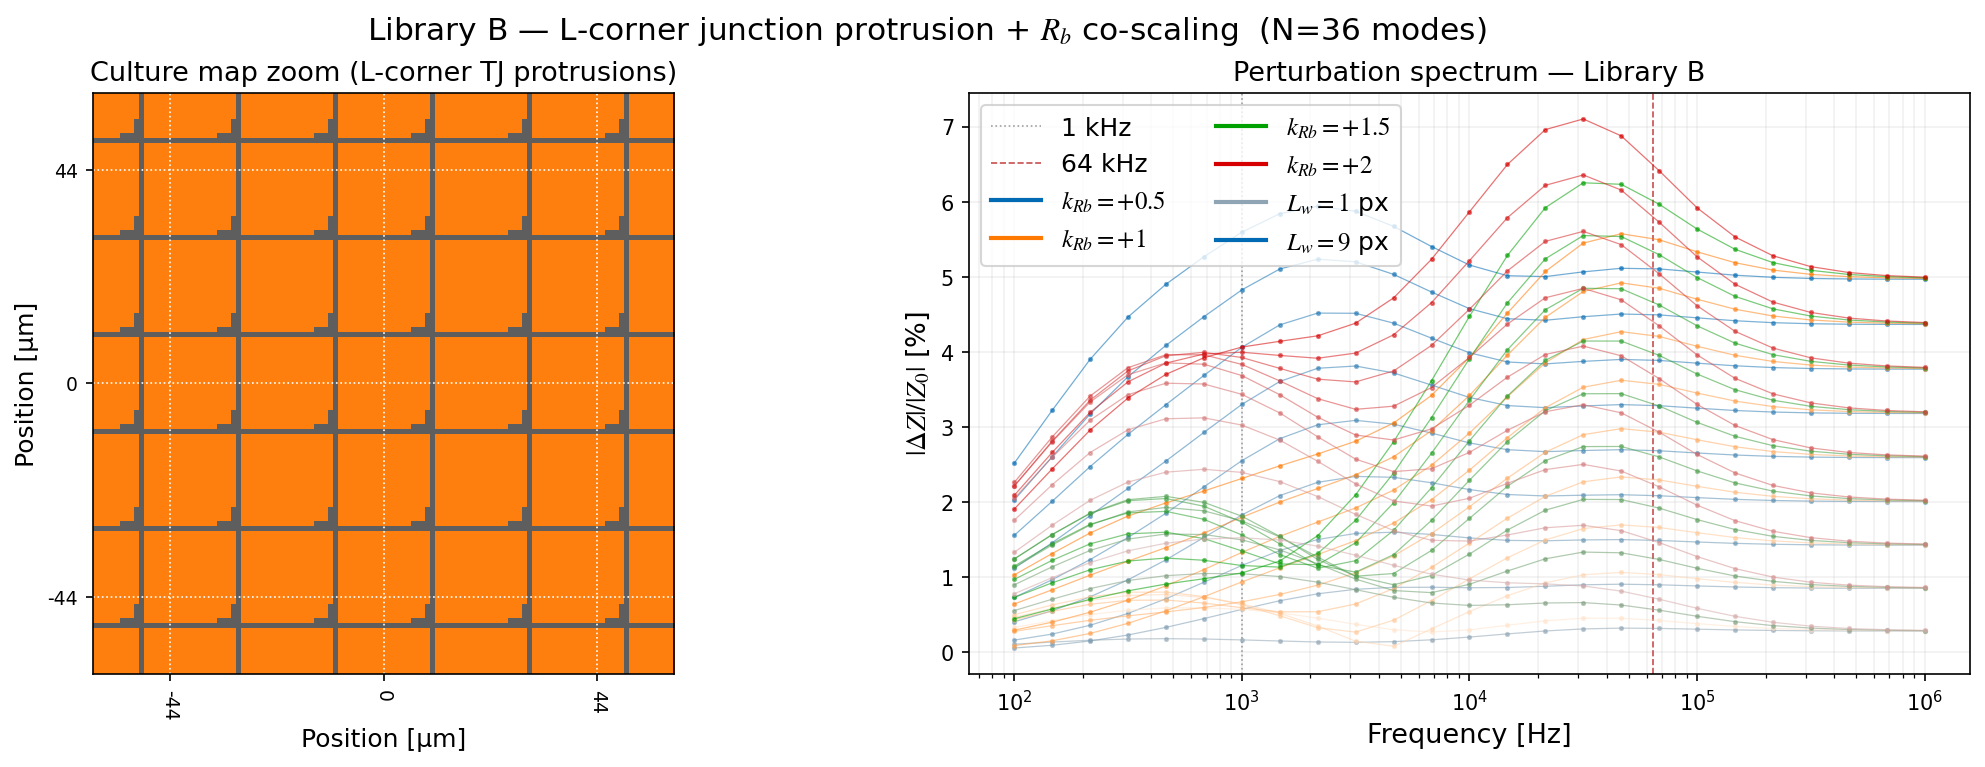
\includegraphics[width=\linewidth]{figure4.png}
 \caption{Library~B: L-corner junction opening with $\Rb$ co-perturbation. \textbf{Left:} Simulation domain zoom showing the L-shaped tight-junction modification in the lower-right corner of each cell, parameterized by arm length $l_w$ and coupling parameter $K_{RB}$. \textbf{Right:} Perturbation amplitude spectrum $|\delta Z|/|Z_0|$ (\%) as a function of frequency for all Library~B modes, spanning the full range of $l_w$ and $K_{RB}$.}
 \label{fig:libB}
\end{figure}

The combined set of library modes must be capable of recreating the experimentally observed micromotion fluctuations. To verify this, the Minkowski sum of the four libraries was computed and its convex hull overlaid on the experimental confluent trajectory in Fig.~\ref{fig:coverage}. The hull delimits the region of the $(\dR,\dX)$ plane accessible to the reconstruction algorithm, although it does not reflect the density of accessible points within that region. It encloses above 99.9\% of every culture experimental trajectory.

\begin{figure}[H]
 \centering
 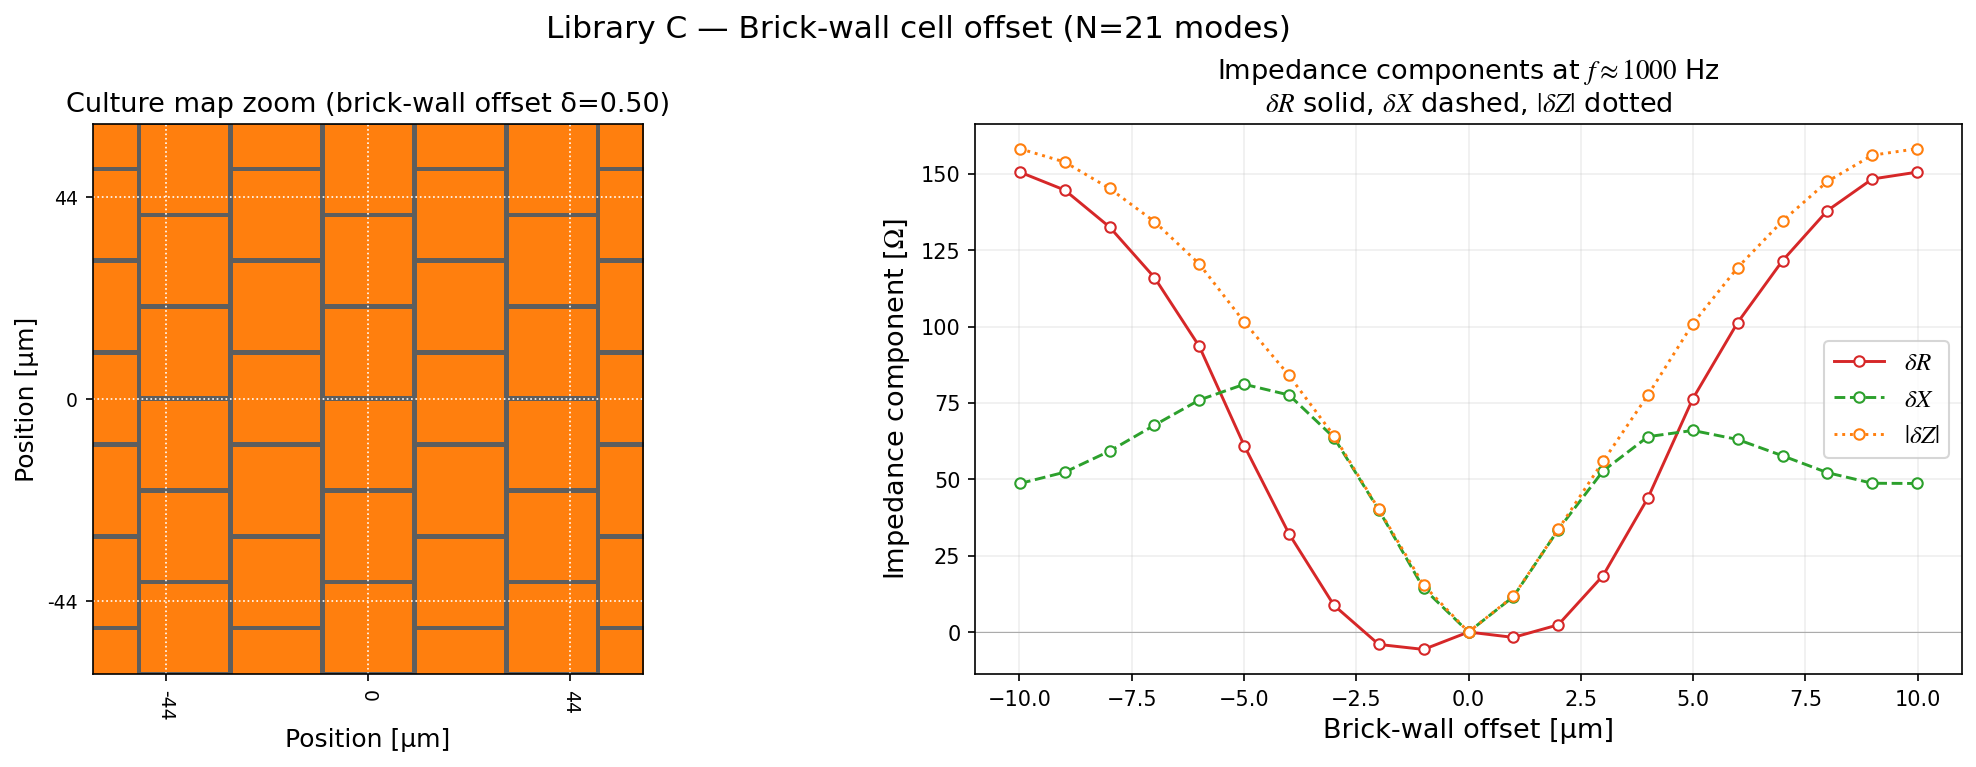
\includegraphics[width=1\linewidth]{figure5.png}
 \caption{Library~C: collective geometric rearrangement from square packing geometry toward a brick-wall pattern without altering individual cell properties. \textbf{Left:} Simulation domain zoom showing maximum brick-wall pattern. \textbf{Right:} Real part $\dR$, imaginary part $\dX$, and magnitude $|\delta Z|$ at \SI{1}{kHz} as a function of vertical displacement.}
 \label{fig:libC}
\end{figure}

\begin{figure}[H]
 \centering
 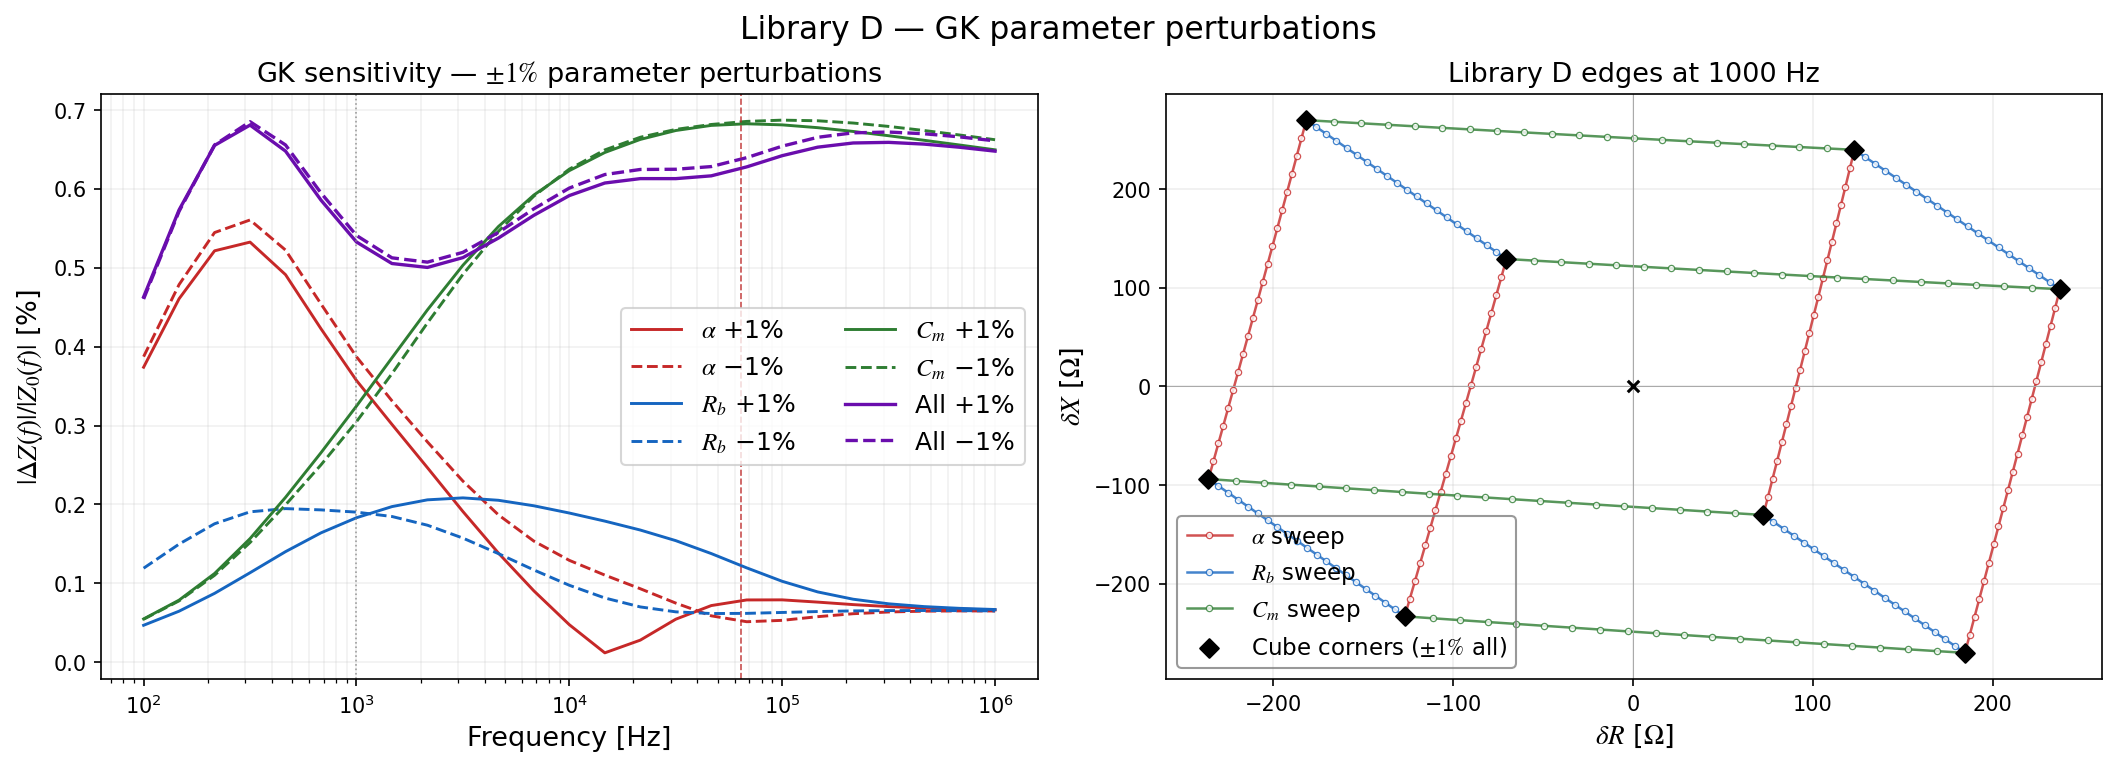
\includegraphics[width=\linewidth]{figure6.png}
 \caption{Library~D, biophysical parameter microperturbation. \textbf{Left:} Individual and combined parameter sensitivity curves showing $|\delta Z|/|Z_0|$ (\%) for $\pm1\%$ perturbations of $\alpha$ (red), $R_b$ (blue), $C_m$ (green), and all three simultaneously (purple). \textbf{Right:} Edges of the perturbation cube projected onto the $(\dR, \dX)$ plane at \SI{1}{kHz}. Each curve sweeps one parameter while the other two are fixed at $\pm1\%$; black diamonds mark the eight cube corners. The interior of the enclosed region contains the remaining modes. Perturbations of $\alpha$ map vertically, $C_m$ horizontally, and $R_b$ diagonally across the plane.}
 \label{fig:libD}
\end{figure}

\begin{figure}[H]
 \centering
 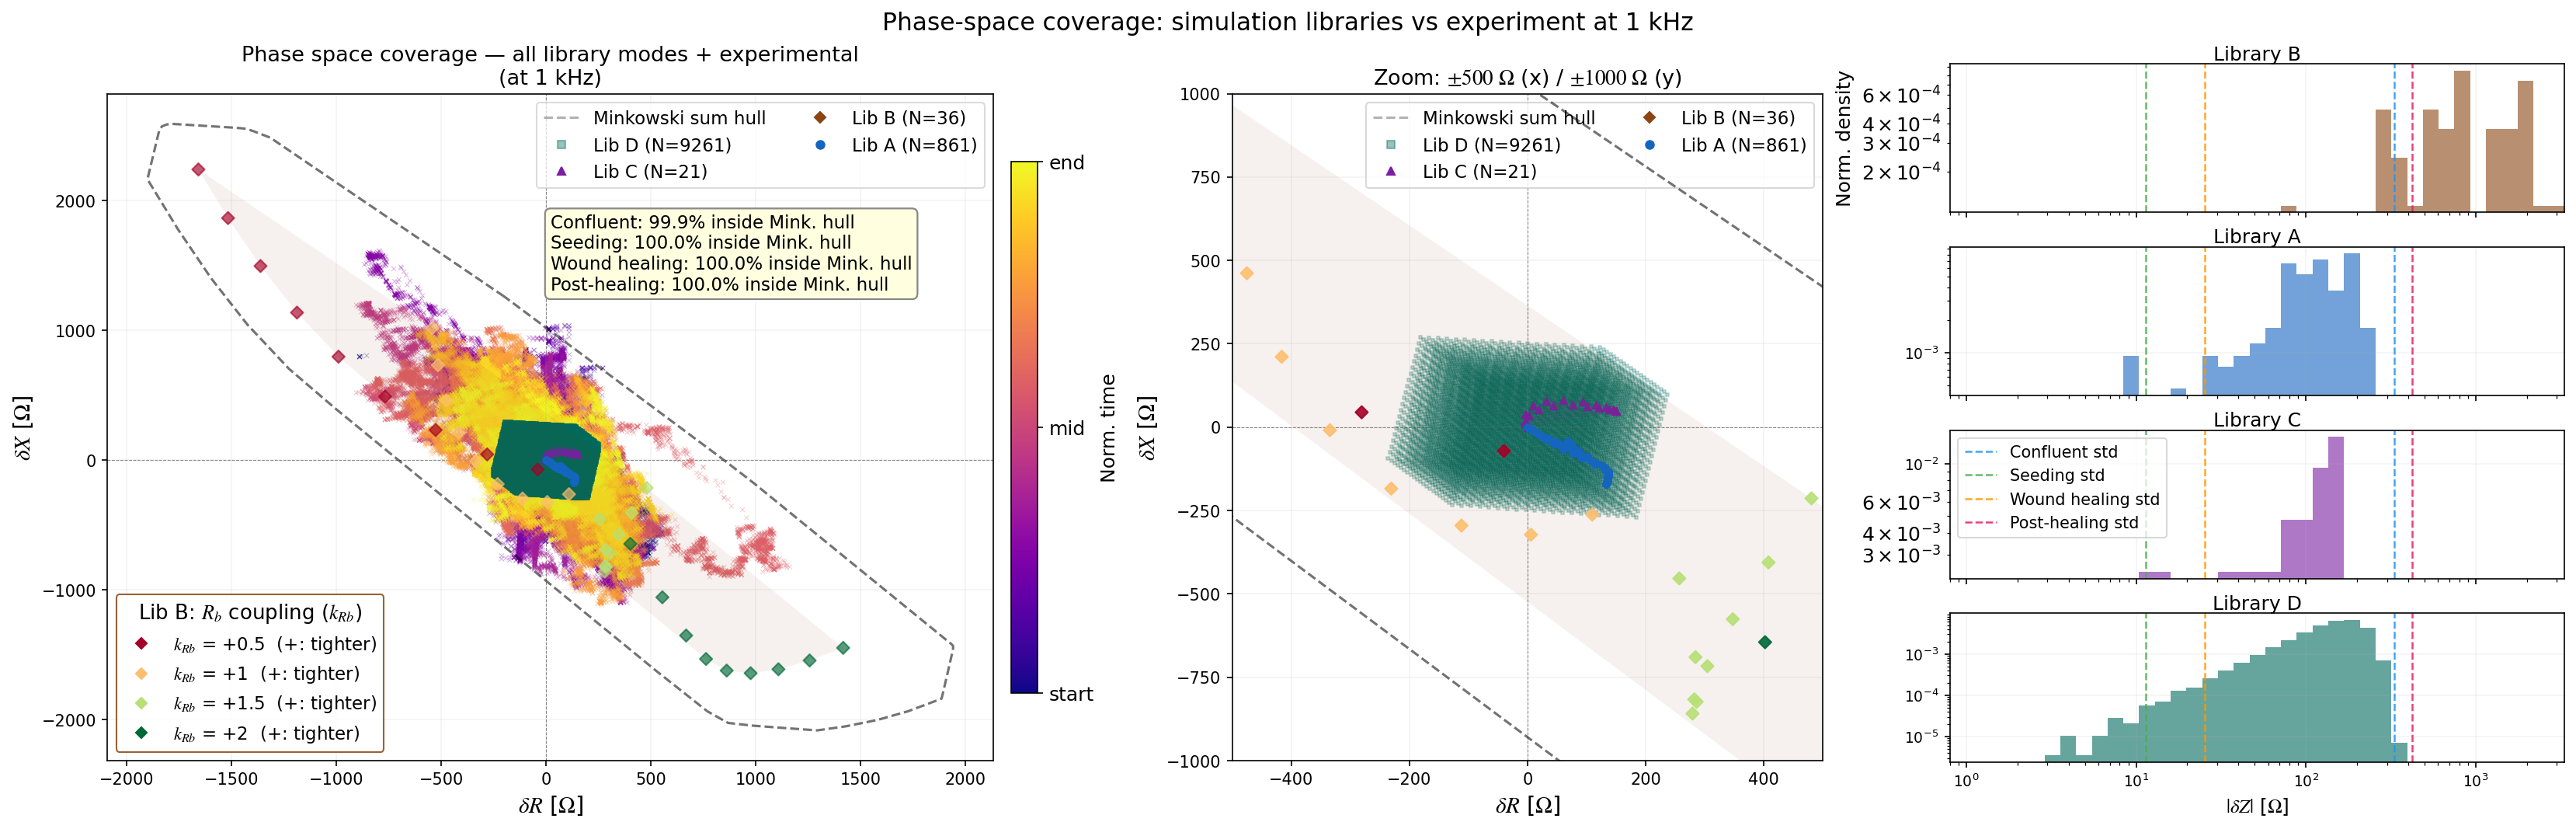
\includegraphics[width=\linewidth]{figure7.png}
 \caption{Phase-space coverage. \textbf{Left:} Scatter $(\dR, \dX)$ of all individual library modes (Libraries~A, B, C, D shown with distinct markers and colors) overlaid with the experimental confluent trajectory. \textbf{Center:} Zoom into the low-amplitude region showing Libraries~A, C, and D. \textbf{Right:} Cumulative distributions of $|\delta Z|$ amplitude, shown separately for each library (one panel per library); vertical dashed lines mark the experimental standard deviations $\sigma_{\dR}$ and $\sigma_{\dX}$ projected onto the amplitude axis.}
 \label{fig:coverage}
\end{figure}

With the libraries defined, the experimental signal $\mathbf{y}(t) = (\delta R(t),\, \delta X(t))^\top \in \mathbb{R}^2$ is decomposed at each time step by a greedy nearest-prototype algorithm. The four libraries are processed in a fixed sequence: B first, then D, A, and finally C, ordered by decreasing phase-space coverage. This sequential procedure is inherently order-dependent; a permutation analysis over all possible orderings showed that the reconstruction quality is primarily determined by placing Library~B first (which occupies a unique, well-separated region of the $(\delta R,\,\delta X)$ plane), while the relative ordering of the remaining three libraries has a modest effect. At each stage the single mode from the current library that minimises the Euclidean distance to the running residual is selected and its $\delta Z$ vector subtracted; after all four libraries have been processed, the remainder $\boldsymbol{\epsilon}(t)$ is the reconstruction residual. Quality is reported as $\mathrm{RMSE}_{\dR}$ and $\mathrm{RMSE}_{\dX}$, the root-mean-square of $\epsilon_R$ and $\epsilon_X$ across all time steps. The reconstruction assigns four labelled physical states per time step, one from each library, constituting a physically interpretable, model-consistent description of the monolayer condition that forms a multivariate time series amenable to further analysis.

As an alternative, a sparse Viterbi algorithm was implemented to enforce temporal continuity in the state sequence~\cite{forney2005viterbi}. The outer sequential structure is identical to the greedy pipeline: the four libraries are processed in the same fixed order on sequential residuals, and the Viterbi regularization is applied independently within each library pass. This does not constitute a global optimization over the joint $\text{B}\times\text{D}\times\text{A}\times\text{C}$ state space, which would be computationally prohibitive. Within each library pass, the per-step nearest-prototype search is replaced by a full dynamic-programming solve over the entire time series, finding the globally optimal state sequence for that library given the current residual (Eq.~\ref{Viterbi}--\ref{eq:trans}). Before each Viterbi pass a null mode ($\delta Z = 0$) is prepended to the library, allowing the algorithm to express that the library contributes nothing at time steps where the residual is already small. The observation cost is the squared Euclidean distance $C_\text{obs}(t,j)=\|\mathbf{r}(t)-\delta\mathbf{Z}_j\|^2$, and the transition cost $T(i,j)$ in Eq.~\ref{eq:trans} is zero when the distance between adjacent modes does not exceed a threshold $\Delta_L$ and infinite otherwise, hard-forbidding large jumps. The distance $d_L$ is library-specific: Euclidean in pixel-displacement space for Library~A; Euclidean in normalised $(K_{Rb},\,l_w)$ space for Library~B; Chebyshev distance in grid-index space for Library~D (to handle the non-uniform parameter grid); and absolute index difference for Library~C.

\begin{equation}\label{Viterbi}
 \{s^*(t)\}_{t=0}^{T-1} = \operatorname*{arg\,min}_{s(t)\in\mathcal{M}_L}
\sum_{t=0}^{T-1} C_\text{obs}(t,\,s(t))
   + \sum_{t=1}^{T-1} T\!\bigl(s(t{-}1),\,s(t)\bigr),
\end{equation}
\begin{equation}\label{eq:trans}
 T(i,\,j) =
 \begin{cases}
   0      & \text{if } d_L(i,j) \le \Delta_L, \\
   \infty & \text{otherwise,}
 \end{cases}
\end{equation}

The libraries were computed for confluent cultures only; the numerical model could in principle simulate partial coverage, but this was deliberately excluded to avoid the combinatorial expansion introduced by randomized cell arrangements on partially covered electrodes. For non-confluent recordings, a calibration factor $\mathit{cal} = |Z_{0,\text{exp}}|/|Z_{0,\text{sim}}|$ is therefore applied as a uniform scalar multiplier to all library mode vectors before reconstruction, correcting for the impedance level offset between the confluent simulation baseline and the experimental state.

\section{Results}
\label{sec:results}

Figure~\ref{fig:eb11_fit} shows the greedy and Viterbi reconstructions of the confluent culture micromotion. Both algorithms track the $\dX$ fluctuation closely, while a systematic $\dR$ residual persists, consistent with the libraries' dominant phase-space direction lying closer to the $\dX$ axis. The greedy reconstruction achieves component-wise RMSE of \SI{34}{\ohm} ($\dR$) and \SI{53}{\ohm} ($\dX$), corresponding to 27\% and 10.2\% of the respective experimental standard deviations. The Viterbi regularization increases both values, and its residual exhibits spikes where the temporal-continuity constraint prevents the algorithm from following rapid experimental excursions.

\begin{figure}[H]
  \centering
  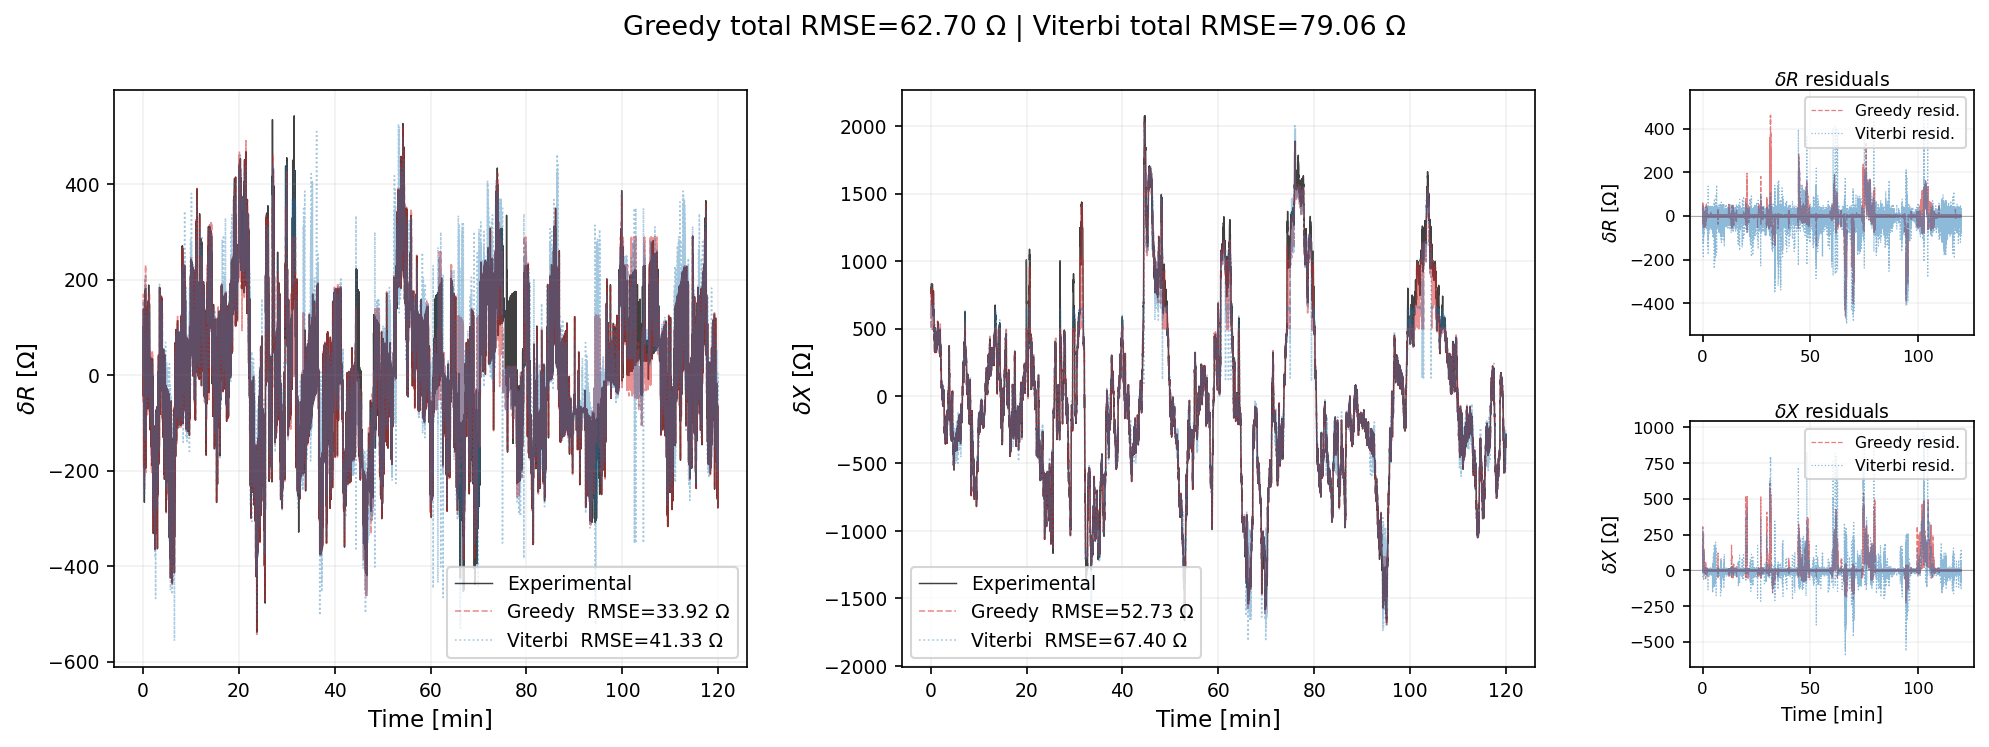
\includegraphics[width=\linewidth]{figure8.png}
  \caption{Reconstruction of impedance fluctuations for the confluent culture (first two hours shown). \textbf{Main panels:} $\dR(t)$ and $\dX(t)$ for the experimental signal (black), the greedy reconstruction (red), and the Viterbi reconstruction (blue). \textbf{Right column:} Corresponding residuals $\epsilon_R(t)$ and $\epsilon_X(t)$. RMSE values in the legend are computed over the complete recording.}
  \label{fig:eb11_fit}
\end{figure}

Table~\ref{tab:rmse} summarizes reconstruction quality for all four experimental cases. The confluent and post-healing electrodes were reconstructed without calibration. Seeding and wound-healing required $\mathit{cal} < 1$, which rescales the library vectors to the lower experimental impedance level, increasing the density of accessible states in the $(\dR,\dX)$ plane. This rescaling reduces the greedy RMSE to below 5\% of $\sigma_{\dR}$ and below 11\% of $\sigma_{\dX}$ for both non-confluent cases, indicating that the perturbation libraries capture the dominant fluctuation mechanisms once the impedance baseline is matched.

\begin{table}[H]
  \centering
  \caption{Reconstruction RMSE for four focus electrodes. Greedy: nearest-prototype; Viterbi: temporal proximity regularization. RMSE in \si{\ohm}; \% relative to experimental standard deviation of each component.}
  \label{tab:rmse}
  \small
  \begin{tabular}{llrrrrrrrrr}
  \toprule
   & & \multicolumn{4}{c}{Greedy} & \multicolumn{4}{c}{Viterbi} \\
  \cmidrule(lr){3-6}\cmidrule(lr){7-10}
  Culture state & cal & $\dR$ [\si{\ohm}] & \%\,$\sigma$ & $\dX$ [\si{\ohm}] & \%\,$\sigma$ & $\dR$ [\si{\ohm}] & \%\,$\sigma$ & $\dX$ [\si{\ohm}] & \%\,$\sigma$ \\
  \midrule
  Seeding        & (0.42) & 0.95 & 4.8  & 0.98 & 10.1 & 3.3  & 16.5 & 2.5  & 25.9 \\
  Confluent      & OFF    & 34   & 27   & 53   & 10.2 & 41   & 32.9 & 67   & 13.0 \\
  Wound healing  & (0.38) & 0.99 & 4.0  & 0.96 &  3.1 & 4.8  & 19.5 & 3.4  & 11.0 \\
  Post-healing   & OFF    & 15.8 & 3.9  & 35.9 &  5.8 & 32.7 &  8.1 & 43.4 &  7.0 \\
  \bottomrule
  \end{tabular}
\end{table}

Figure~\ref{fig:mode_states} summarizes the per-library state sequences selected by each algorithm for the confluent recording. The left and central columns show the greedy and Viterbi temporal evolution of each parameter over the first two hours, respectively. The right column overlays both algorithms within a 5-min zoom window centered on the peak $|\dR_{\mathrm{exp}}|$ event.

The $(K_{Rb}, l_w)$ scatter (Library~B) shows that both algorithms sample the same discrete set of configurations throughout the displayed interval. This is consistent with Fig.~\ref{fig:coverage}, since these modes provide the coarse correction for confluent cultures. Library~D parameter distributions are not statistically different between the two algorithms: $\delta\alpha$ is skewed toward $-1\%$, $\delta R_b$ shows a broad distribution across mid-range values with pronounced peaks at the perturbation extremes, and $\delta C_m$ is centered around zero. Moreover, the Viterbi zoom reveals an anticorrelation between $\delta\alpha$ and the other two parameters, indicating that the reconstruction consistently opposes the sign of the cleft-geometry perturbation to those of the junction-resistance and membrane-capacitance perturbations. The displacement distribution (Library~A) is markedly different between the two algorithms. The greedy distribution is multimodal, reflecting the algorithm's freedom to jump between discrete regions of the shift library at each time step. The Viterbi solution is dominated by a single population near zero displacement, with occasional selection of the library boundary or its symmetric counterpart at the first negative displacement values. This contrast reflects the temporal-continuity penalty against large jumps, which forces Viterbi to choose one stable regime and remain near it. The brick-wall offset (Library~C) distribution is dominated by few recurrent modes. These narrow occupancy are a direct consequence of Library~A and C prominent phase~space direction and being processed last in the fitting sequence.

The temporal zoom panels make the algorithmic contrast explicit: the greedy traces switch rapidly between library modes at every time step, achieving the per-step optimum, while the Viterbi traces exhibit piecewise-constant plateaus separated by discrete transitions. Neither algorithm produces physically implausible states, as both are constrained to the pre-computed library modes.


As a consistency check on whether the discrete mode representation preserves the temporal correlation structure of the signal, the fractal dimension of each reconstructed series was compared to its experimental counterpart. Table~\ref{tab:fractal_comparison} shows agreement within windowed uncertainty for all culture states and both algorithms under the Higuchi estimator. The largest departure appears in the post-healing Viterbi $\dX$ under R/S estimation ($d_f = 1.51(3)$ vs.\ experimental $1.38(3)$), attributable to the piecewise-constant nature of the Viterbi solution, whose discrete transitions between library states introduce artificial scale breaks that the R/S estimator interprets as increased complexity.

\begin{table}[H]
  \centering
  \caption{Fractal dimension single-slope $d_f$ — experimental and reconstructed
   signals ($\delta R$ and $\delta X$). Values are mean with windowed standard
   deviation in parentheses.}
  \label{tab:fractal_comparison}
  \scriptsize
  \begin{tabular}{lcccccc}
  \toprule
   & \multicolumn{6}{c}{$\delta R\,/\,\delta X$} \\
  \cmidrule(lr){2-7}
  Culture state & \multicolumn{3}{c}{Higuchi} & \multicolumn{3}{c}{R/S} \\
  \cmidrule(lr){2-4}\cmidrule(lr){5-7}
   & Experimental & Greedy & Viterbi & Experimental & Greedy & Viterbi \\
  \midrule
  Seeding       & $1.87(3)/1.920(6)$ & $1.88(3)/1.920(6)$ & $1.88(3)/1.921(7)$  & $1.80(2)/1.78(2)$  & $1.79(2)/1.78(2)$  & $1.76(2)/1.78(2)$ \\
  Confluent     & $1.81(3)/1.43(3)$  & $1.81(3)/1.45(3)$  & $1.81(3)/1.47(3)$   & $1.74(3)/1.43(4)$  & $1.75(3)/1.47(3)$  & $1.74(2)/1.53(3)$ \\
  Wound healing & $1.86(3)/1.78(10)$ & $1.86(3)/1.78(10)$ & $1.85(4)/1.79(10)$  & $1.78(3)/1.66(8)$  & $1.79(3)/1.66(8)$  & $1.76(4)/1.66(8)$ \\
  Post-healing  & $1.67(4)/1.40(2)$  & $1.67(4)/1.41(2)$  & $1.70(4)/1.45(2)$   & $1.43(4)/1.38(3)$  & $1.44(4)/1.39(3)$  & $1.54(4)/1.51(3)$ \\
  \bottomrule
  \end{tabular}
\end{table}


\begin{figure}[H]
  \centering
  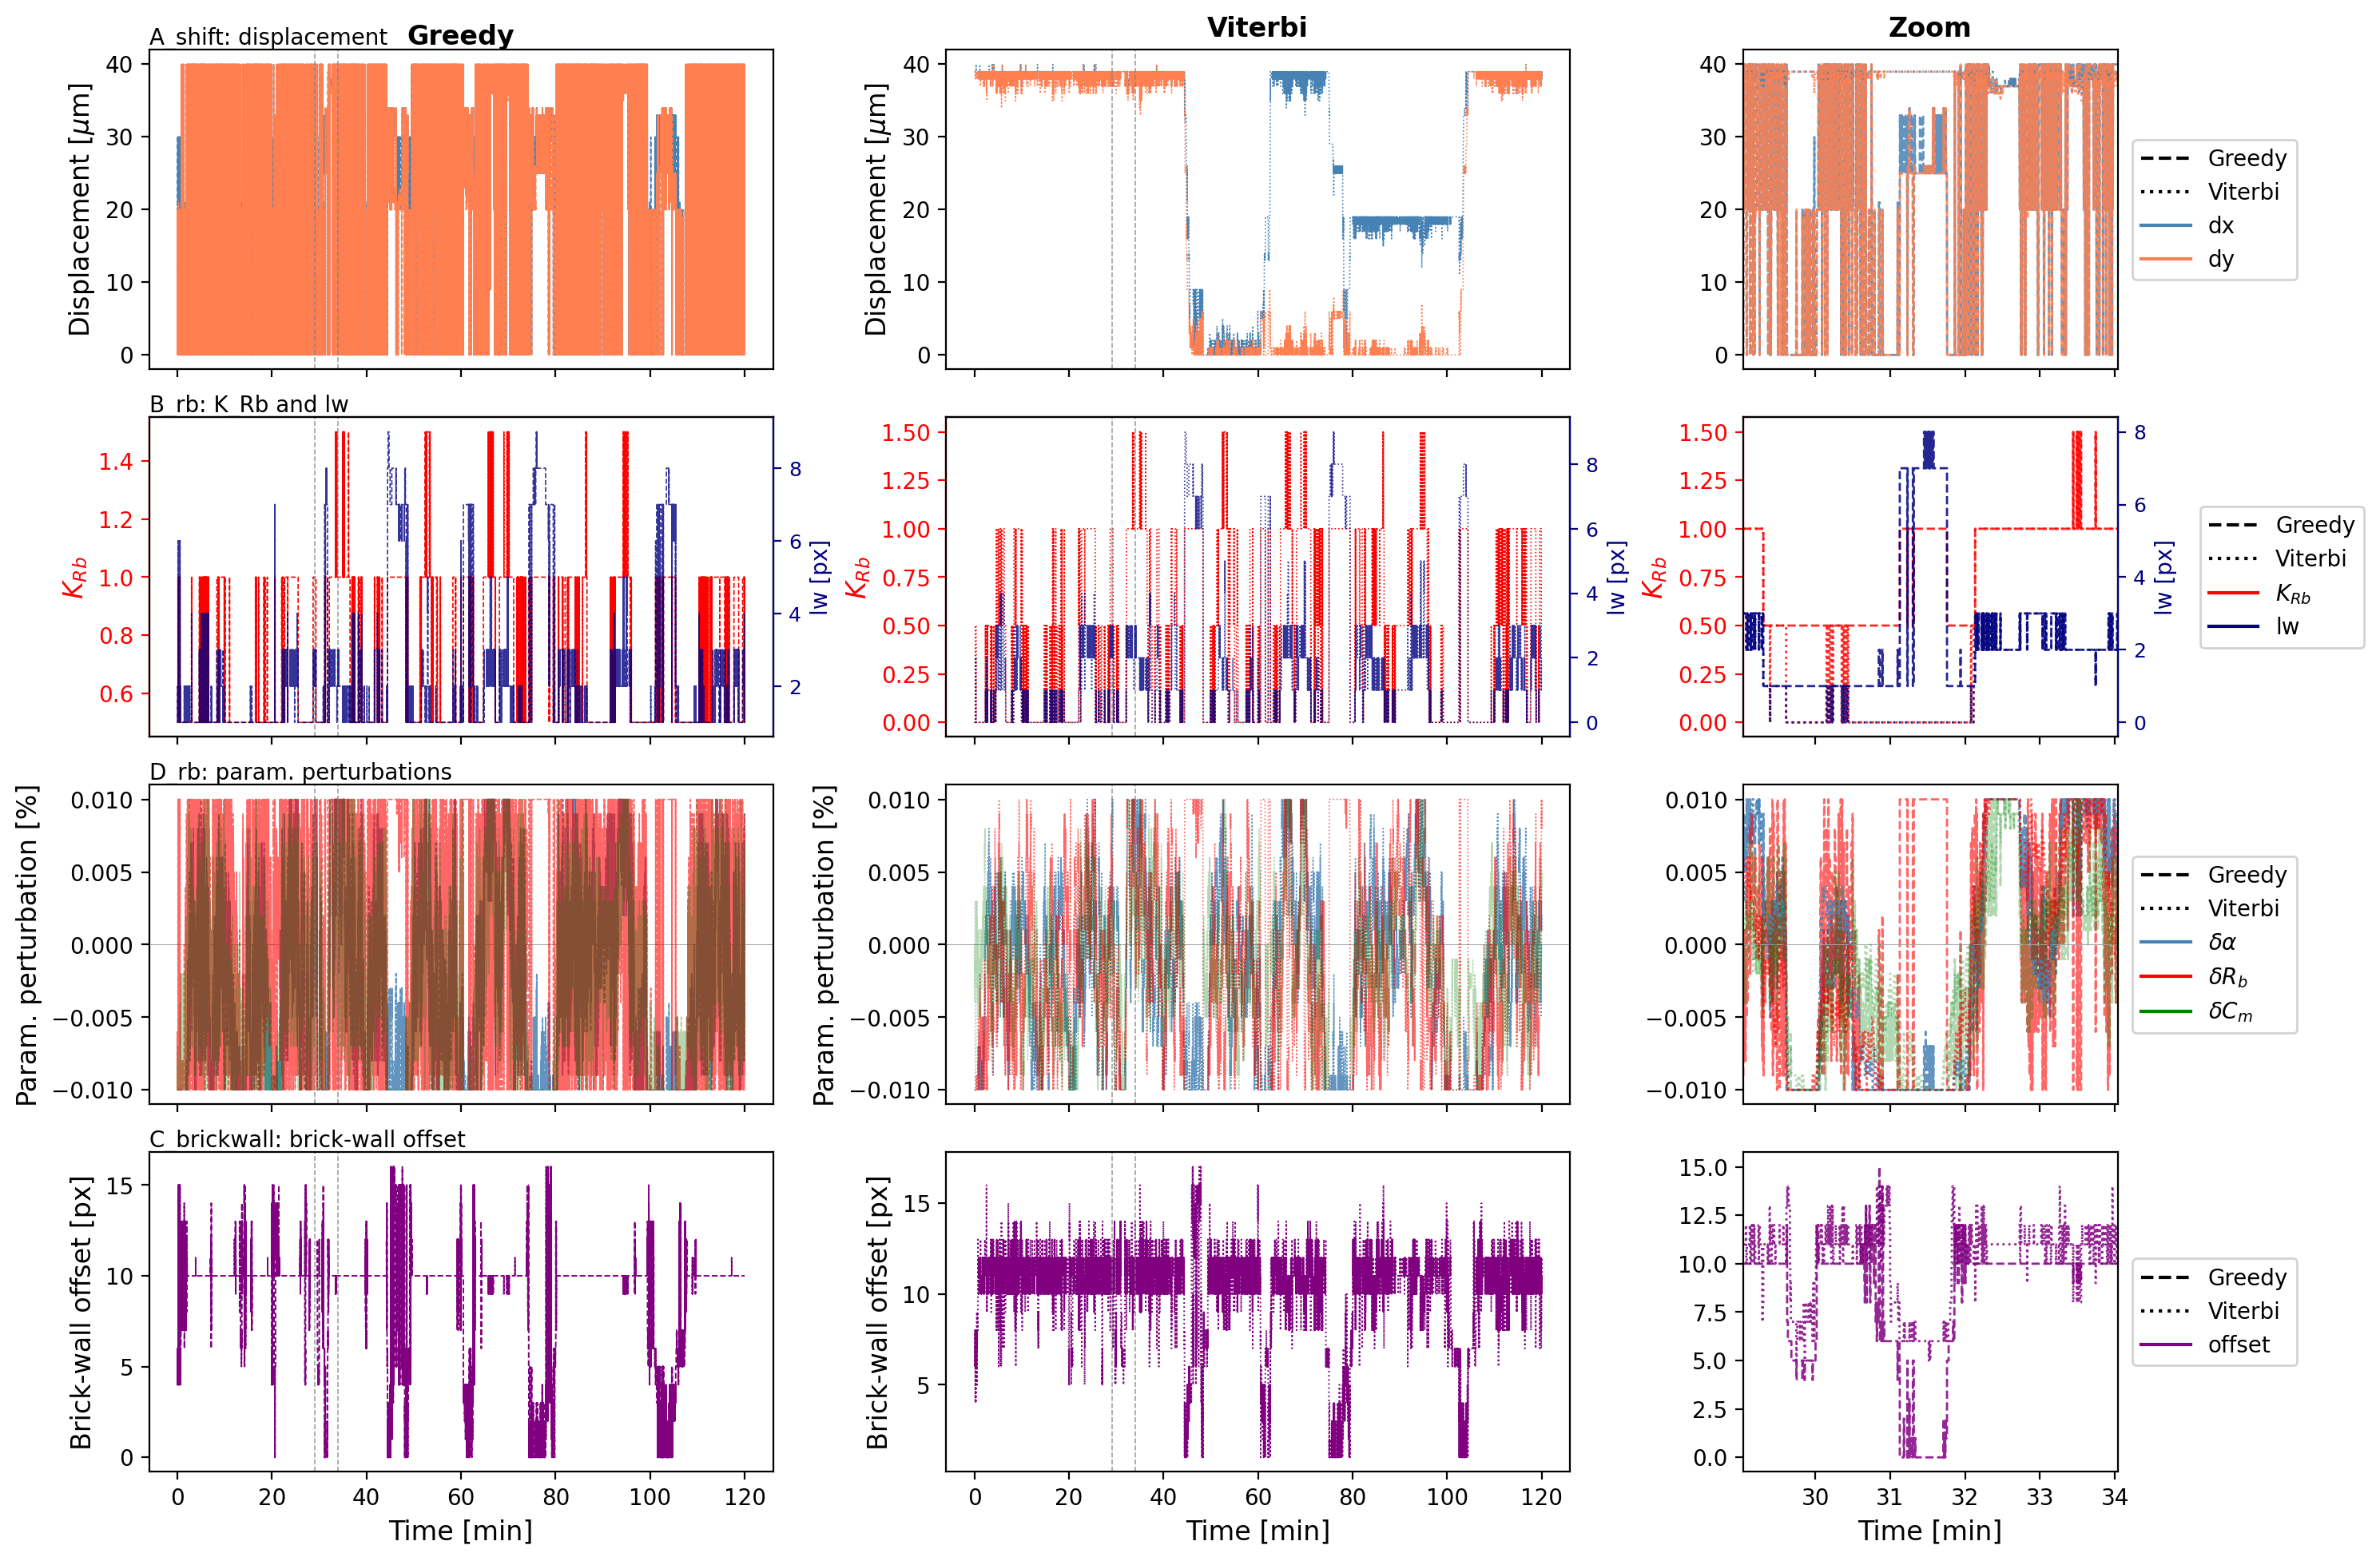
\includegraphics[width=\linewidth]{figure9.png}
  \caption{Per-library state sequences for the confluent recording. \textbf{Left and center columns:} temporal evolution of each library parameter over the first two hours for the greedy and Viterbi algorithms, respectively. Rows from top to bottom: Library~A displacement $(dx, dy)$; Library~B $(K_{Rb}, l_w)$; Library~D fractional perturbations $(\delta\alpha, \delta R_b, \delta C_m)$; Library~C brick-wall offset. \textbf{Right column:} 5-min zoom window centered on the peak $|\dR_{\mathrm{exp}}|$ event, with both algorithms overlaid.}
  \label{fig:mode_states}
\end{figure}


% ══════════════════════════════════════════════════════════════════════════════% ══════════════════════════════════════════════════════════════════════════════
\section{Conclusions }

The pipeline demonstrated here decomposes ECIS micromotion time series into model-consistent perturbation modes from four deterministic libraries, assigning a labelled physical state per library at each time step. The greedy nearest-prototype algorithm achieves the minimum available RMSE, while the Viterbi temporal-proximity regularization enforces smoother state trajectories at the cost of fit quality, reflecting a fundamental trade-off between fit fidelity and temporal coherence. As a consistency check, the fractal dimension of the reconstructed signals agrees with that of the experimental signals within windowed uncertainty for all culture states and both algorithms, indicating that the discrete mode representation preserves the temporal correlation structure of the micromotion signal. This agreement demonstrates signal-level reconstruction fidelity and preservation of statistical scaling properties, but does not by itself validate the biological identity of the assigned perturbation modes.

The per-library state distributions provide a window into the dominant physical mechanisms driving micromotion in each culture scenario. For the confluent monolayer, Libraries~B and~D (tight-junction geometry and biophysical parameter drift) are the principal contributors, indicating that micromotion is driven primarily by fluctuations in junction resistance and small-amplitude parameter drift, consistent with homeostatic barrier maintenance. In the seeding recording, Library~A occupancy broadens relative to the confluent case, reflecting a larger contribution from lateral cell displacement, consistent with cells that have not yet established firm substrate adhesion. During wound healing, Library~D exhibits an anticorrelation between $\delta\alpha$ and ($\delta R_b$, $\delta C_m$), suggesting that cells simultaneously tighten the cell-substrate cleft while stiffening paracellular junctions, a signature consistent with cytoskeletal contractility during active migration. The post-healing monolayer shows the narrowest mode occupancy across all libraries and the lowest fractal dimension, indicating a mechanically quiescent state with reduced micromotion complexity following wound closure and radial cell reordering. These interpretations are model-consistent inferences from the decomposition; independent biological validation through pharmacological perturbations (e.g., cytochalasin~D for cytoskeletal disruption, EGTA for junction opening) remains a direction for future recordings to analyze.

The calibration factor required for non-confluent recordings (seeding and wound-healing) exposes a limitation of the current library design. Because the libraries were computed for a fully confluent baseline, partially covered electrodes are represented by rescaling the perturbation amplitudes rather than by modifying the underlying geometry. This approximation is self-consistent within the linear-perturbation regime but does not capture the qualitatively different micromotion dynamics expected at low confluence, where individual cells behave as isolated particles rather than coupled elements of a collective. Extending the library construction to include partially covered electrode configurations would remove this approximation and allow direct reconstruction of the seeding and wound-healing phases without amplitude calibration. A further limitation is that all four libraries apply collective perturbations, where every cell receives the same parameter change, so individual, spatially heterogeneous cell movements are not captured. Incorporating spatially distributed perturbations, potentially guided by statistical distributions of cell-level parameter values, is a natural extension that would increase the physical realism of the decomposition.

The sensitivity of the ECIS measurement to micromotion perturbations is frequency-dependent through the GK dispersion relations. Analysis of the library sensitivity curves shows that the perturbation amplitude $|\delta Z(f)|$ peaks for most libraries in a frequency band approximately between \SI{1}{\kilo\hertz} and \SI{3}{\kilo\hertz}. Below this band, the CPE electrode response dominates, and above it, the constriction resistance dominates, both resulting in decreasing sensitivity to cellular perturbations. This sensitivity band is specific to the MDCKII cell line on the 96W1E+ electrode array and the associated biophysical parameters; different electrode geometries, electrolyte interfaces, or cell types would shift the optimal frequency range. The \SI{1}{\kilo\hertz} excitation used in the analyzed dataset therefore sits near the sensitivity maximum, which contributes to the high quality of the reconstruction but also implies that moving to other frequencies would not improve the signal-to-noise ratio of the micromotion component. Nevertheless, to further improve the precision and reach of this pipeline, future measurements require acquisition protocols that alternate between culture spectral impedance and micromotion monitoring, since each library mode has a precomputed spectral impedance response. If the experimental system provides impedance measurements at multiple frequencies, the search can be conducted in a higher-dimensional observation space, substantially restricting the set of admissible modes and resolving the phase-space overlap that limits single-frequency reconstruction. Furthermore, spectral shape information provides a physically motivated constraint on which library modes can be consistent with a given experimental state, enabling mode pre-filtering before the search and improving physical interpretability.

Taken together, this work establishes a proof of concept: ECIS micromotion fluctuations can be decomposed into physically interpretable contributions using entirely deterministic, pre-computed simulation libraries, without any stochastic model component. The current single-frequency, collective-perturbation framework already reconstructs the experimental signal and preserves its fractal scaling, while revealing culture-state-dependent mechanisms. The path toward higher fidelity is clear with dual-measurements that provide spectral impedance sweeps and single-frequency micromotion acquisition would enable multi-frequency reconstruction, resolving the degeneracies inherent in two-observable decomposition and bringing the pipeline closer to unique mode identification.

\bibliographystyle{unsrt}
\bibliography{bibliography}

\end{document}
